\def\T{{\cal T}}
\def\X{{\cal X}}
\def\Q{{\cal Q}}
\def\R{{\mathbb R}}
\def\U{{\mathcal U}}
\def\M{{\mathbf M}}
\def\N{{\mathbb N}}
\def\R{{\mathbb R}}
\def\E{{\mathbb E}}
\def\U{{\mathcal U}}
\def\G{{\mathcal G}}
\def\Z{{\mathcal Z}}
\def\X{{\mathcal X}}
\def\C{{\mathcal C}}
\def\I{{\mathbf I}}
\def\P{{P}}
\def\K{{\mathbf K}}
\def\Y{{\mathbf Y}}
\def\z{{\mathbf z}}
\def\t{{\mathbf t}}
\def\u{{u}}
\def\w{{\mathbf w}}
\def\g{{\mathbf g}}
\def\bp{{\bm\phi}}
\def\L{{\cal L}}

%---------------------------------------------------------------------------------
\chapter{Image Ranking by Non-Parametric Kernel Learning}
\label{chp:application}
%---------------------------------------------------------------------------------

Kernel methods have become one of the state-of-the-art methods in nowadays machine learning community and have been applied to a variety of applications. In this thesis, we study two important applications: image re-ranking with non-parametric kernel \cite{civr/ZhuangH10} and social streng modeling with multiple kernel learning to rank \cite{mm/ZhuangMHHL11}.

%%=====================================
%\section{Image Ranking by Non-Parametric Kernel Learning}
%%=====================================

Social image retrieval has become an emerging open problem in web
image search. In this chapter, we address the challenge of text-based social
image retrieval, which aims to identify a set of relevant social images
related to a text-based query from a corpus of social images. Regular
approaches for social image retrieval simply adopt typical text-based
image retrieval techniques for retrieving the relevant social images based
on the associated tags, which may suffer from noisy tags. In this chapter, we
present a novel nonparametric kernel learning framework for social image
ranking, which explores both textual and visual contents of social images
for improving the ranking performance of social image retrieval tasks.
Unlike existing methods that often adopt some fixed parametric kernel
function, our framework learns a nonparametric kernel matrix that can
effectively encode the information from both visual and textual domains.
Although the proposed learning scheme is transductive, we suggest some
solution to handle unseen data by warping the nonparametric kernel space
to some input kernel function. Encouraging experimental results on
real-world social image data exhibit the effectiveness of the proposed
method.

Along with the popularity of various digital imaging devices and the advances of Internet technologies, more and more digital images and photos have been uploaded and shared on the World Wide Web. Unlike the situation of one decade ago, web images are playing a more and more important role nowadays. Web image search has become an active yet very challenging research problem.

One major difficulty for web image search is that most images are usually not
annotated with proper tags, and many of them are even completely unlabeled. In addition, even for the annotated images, the associated tags could be noisy, irrelevant, and often incomplete for describing the contents of the images. This poses a challenge for typical approaches of web image search used by existing web search engines, which often simply apply regular text based retrieval techniques on web image search domains.

One possible direction to improve existing text-based web image search approaches is to explore the techniques of content-based image retrieval (CBIR)~\cite{pami/SmeuldersWSGJ00,pami/SmeuldersWSGJ00}, which has been extensively studied in multimedia communities in the past decade. While CBIR techniques are able to retrieve images based on the low-level visual contents, one main drawback of CBIR lies in the difficulty of finding/drawing an appropriate query example for describing the user's search intention. This is probably why query-by-text image retrieval methods remain the most popular approach despite that their ordinary performance is far from perfect.

Instead of directly applying CBIR techniques, another alternative approach for
improving the performance of text-based image retrieval is to investigate automatic image annotation techniques, which aims at annotating a web image with a set of relevant tags automatically. While automatic image annotation has been actively studied and shown to be able to improve the performance of text-based image retrieval in a small-scaled experimental testbed, it remains unknown for the effectiveness and scalability of the related techniques when being deployed in a massive scale environment, such as WWW images.

Recently, there is some emerging study for improving a text-based web image
retrieval task by implicitly exploring the visual content without using query image examples~\cite{pami/JingB08}. They proposed a visual re-ranking method, termed ``VisualRank", which is an extension of PageRank~\cite{cn/BrinP98} by exploiting the visual information in the web image ranking task. Although encouraging results had been shown for improving regular text-based web image search, the VisualRank
approach adopts a rigid visual similarity measure approach, which may suffer from the well-known challenge of semantic gap between low-level visual features and high-level semantic concepts~\cite{pami/SmeuldersWSGJ00}. This motivates our study in this chapter, which aims to improve VisualRank by a novel nonparametric kernel ranking scheme.

Besides, unlike previous studies on web image retrieval, our study
considers {\it social images}, which are uploaded and shared by web users
in social web sites. In contrast to generic web images, social images have
rich user-generated contents, including tags provided by web users.
Despite the good quality tags, noise remains an unavoidable issue for
social image retrieval. Here our goal is to improve the
performance of text-based social image retrieval by mining rich tag and
visual contents through a novel nonparametric kernel based ranking
approach.

In particular, our framework differs from the previous approaches that often assume some fixed kernel function for similarity measure. We propose to learn an optimized kernel from the rich annotated social images, aiming to bridge the semantic gap towards effective image similarity measure. To the best of our knowledge, this is the first kernel learning approach that learns to optimize a kernel for a web image ranking task.

As a summary, the key contributions of this chapter include:
\begin{itemize}
  \item We propose a novel nonparametric kernel ranking framework that aims to learn an optimized kernel from both textual tag information and visual contents of social images;

  \item We present an efficient algorithm for nonparametric kernel ranking, which can efficiently learn nonparametric kernels for improving the VisualRank performance in a text-based social image retrieval task.

  \item We conduct an empirical study for comparing the proposed algorithm with the state-of-the-art method on a large-scale social image repository.

\end{itemize}

The rest of this section is organized as follows. Section \ref{sec:rerank-framework} reviews some preliminaries of the VisualRank~\cite{pami/JingB08} framework, in which a similarity matrix plays a central role. Section~\ref{sec:rerank-kernel-learning} presents the proposed nonparametric kernel learning technique for learning kernels from social images, and studies its application for improving text-based social image retrieval tasks. Section \ref{sec:rerank-experiment} gives our empirical study.


%========================================================================
\section{Problem Setting} \label{sec:rerank-framework}
%========================================================================

In general, a social image often contains rich contents, including user-generated tags, visual content, rating, etc. In our approach, we simplify the social image representation by considering only visual content and user-generated tags. Specifically, a social image is represented as $z_i=(x_i,t_i)$, where $x_i\in\mathcal{X}$ denotes the vector of its visual content, and $t_i\in\mathcal{T}$ denotes the vector of its associated tags. We further assume that the query space $\Q$ shares the same vocabulary space with the tag space $\mathcal{T}$, i.e., $\T :=\Q$.

Consider a social image retrieval task, given some text-based query $q\in\Q$, our goal is to retrieve and rank the relevant social images from a social image repository $\mathcal{D}=\{z_i=(x_i,t_i),i=1,\ldots,n\}$. Specifically, let us denoted $\mathcal{R}(q)$ and $\overline{\mathcal{R}}(q)$the set of relevant and irrelevant social images related to query $q$ respectively, the objective of the social image retrieval task is to find some ranking function $f:\mathcal{X}\times\mathcal{T}\rightarrow\mathcal{R}$ such that $f(z_i)>f(z_j)$ for any two images $z_i\in\mathcal{R}(q)$ and $z_j\in\overline{\mathcal{R}}(q)$.

Most approaches for web image retrieval by existing web search engines often formulate the ranking function $f$ by adopting some text-based retrieval model to rank the web images according to the associated tags. While these approaches are efficient by taking advantage of effective text indexing techniques, their ranking performance is not be always satisfied due to the noisy textual content that is common for WWW images. To address this challenge, the recent study~\cite{pami/JingB08} has proposed a visual re-ranking method for improving the web image search performance. Next we briefly review the Visual Ranking method.

%========================================================================
\section{VisualRank for Web Image Search}
%========================================================================

The key idea of VisualRank~\cite{pami/JingB08} was adapted from the intuition of PageRank~\cite{cn/BrinP98}, i.e., images similar to a relevant image are also relevant. Specifically, suppose we have a similarity matrix $K$, where $K_{ij}$ is the visual similarity between image $x_i$ and $x_j$. If the entry $K_{ij}$ has a large value, we deem that $x_i$ supports the importance of $x_j$ to a large extent. Therefore, by exploiting the visual information between pairs of images, we re-rank the images and hopefully improve the accuracy of retrieval results of text-based methods.


Let $VR \in \mathbb R^n$ be the ordering score of $n$ social images. A larger score indicates the image is more relevant, thus resulting a higher position in the ranking result. The VisualRank (VR) is iteratively defined as:
\[
VR = K \times VR,
\]
where $K$ is a normalized matrix such that $0\leq K_{ij} \leq1$ and each column sums to 1. When $K$ is symmetric, it becomes a doubly stochastic matrix~\cite{HornJ85}. From a random walk perspective, $K_{ij}$ measures the probability of $z_i$ randomly travels to $z_j$. Typically, a damping factor $\lambda_d$ is introduced to incorporate some prior ranking score $P$:
\[
VR = \lambda_d K \times VR + (1 - \lambda_d) P, \mbox{where}\; P = \left[\frac{1}{n}\right]_{n\times 1}
\]

The key to VisualRank is how to find a good similarity matrix $K$. The regular approach~\cite{pami/JingB08} is to simply calculate the similarity/distance matrix based on visual contents $\mathcal{X}$ (either local or global visual features) extracted from the images. Such an approach falls short when the visual similarity is not very effective, which is possible primarily due to the well-known semantic gap between low-level visual features and high-level semantic concepts. To address the limitation of the regular VisualRank approach, in this thesis, we present a novel nonparametric kernel ranking framework, which aims to learn a good visual kernel $K$ that best preserves the semantics by exploiting both visual and textual contents.

%========================================================================
\section{Nonparametric Kernel Ranking for Social Image Retrieval} \label{sec:rerank-kernel-learning}
%========================================================================

In this section, we present a novel nonparametric kernel ranking method for social image retrieval. The key idea is to improve VisualRank by learning an optimized visual kernel.

%========================================================
\subsection{Learning Semantics-Preserving Kernels}
%========================================================

The goal of our task is to learn a visual kernel $K\in\mathbb{S}_+^{n\times n}$ for measuring similarity $k(z_i,z_j)$ between any two social images $z_i$ and $z_j$,
which best preserves the semantics by exploring both textual and visual contents.

The first concern of our kernel learning task is how to effectively explore the textual
contents of social images. One approach to this challenge is to optimize $K$ by
maximizing the dependance between the two domains $\mathcal{X}$ and ${T}$. To
this send, we suggest to employ the Hilbert-Schmidt Independence Criterion
(HSIC)~\cite{alt/GrettonBSS05} for the dependence measure between $\mathcal X$
and $\mathcal T$, which is defined below.

\begin{definition}[Empirical HSIC]
Let us denote by $Z=\{(x_1,t_1),\ldots,(x_n,t_n)\}$ a collection of $n$ independent observations drawn from the joint distribution $\mathcal{X}$ and $\mathcal{T}$, an estimator of HSIC is given by
\[
\mathrm{HSIC}(Z,\mathcal X, \mathcal T) = \frac{1}{(n - 1)^{2}} \tr K H K_t H,
\]
where $K$ and $K_t$ refers to the kernel matrices in visual space and textual space respectively, and $H=I-\frac{1}{N}\mathbf{1}_N\mathbf{1}_N^{\top}$.
\end{definition}

The HSIC measures the dependence between two random variables
$x\in\mathcal{X}$ and $t\in\mathcal{T}$ by computing the square of the norm of the cross-covariance operator over the domain $\mathcal X \times \mathcal T$ in Hilbert Space. One can show the norm vanishes on the condition that $x$ and $t$ are independent. A large value of HSIC indicates a strong dependence with respect to the choice of the kernels. If we ignore the centering matrix $H$, it coincides with the concept of kernel target alignment~\cite{nips/CristianiniSEK01}. It has been successfully applied in some recent machine learning work~\cite{nips/SongSBG07}.

In addition to the tag information, we expect the kernel $K$ should also encode the information of visual features. Combining the empirical HSIC and the visual feature concern, we formulate the semantics-preserving kernel learning problem as a nonparametric kernel learning task:
\begin{eqnarray} \label{eqn:tk-obj}
&\max_{K}& \tr K H K_t H\\
&\mbox{s.t.}& K_{ii} + K_{jj} - 2K_{ij} \leq d^2_{ij}\;\;\forall (i, j) \in \mathcal N, \nonumber\\
&& K \subset \mathbb S^{N \times N}_+,\nonumber
\end{eqnarray}
where $\mathbb S^{n \times n}_+$ denotes the space of positive semi-definite cones,
and $\mathcal N$ is a set of all pairs $(i, j)$ where $x_i$ and $x_j$ are close to each
other according to their visual distance, which is empirically obtained by checking if
they are among each other's $k$ nearest neighbors based on some metric defined on
the visual space $\mathcal X$.

{\bf Remark.} Unlike a regular fixed kernel (e.g. RBF kernel) defined on visual space $X$, the above formulation finds an optimized kernel $K$ by (1) exploring the textual contents through $K_t$ and (2) encoding the visual information by enforcing the constraints according to the visual distance $d_{ij}$ in a unified framework that can effectively overcome the semantic gap challenge.

%========================================================
\subsection{Efficient Kernel Learning Algorithm}
%========================================================

The optimization of (\ref{eqn:tk-obj}) is an SDP problem, which in general has to be solved in time complexity of $O(n^6)$ by a regular SDP solver. This intensive computation cost prohibits its application to large-scale real applications. To address this challenge, we propose an efficient algorithm that adopts a special SDP solver to explore the problem structures.

First of all, we notice that it may be too strong to enforce all distance constraints
satisfied in the optimization problem (\ref{eqn:tk-obj}). We reformulate the
optimization by introducing slack variables $\xi$ (that are similar to the approach is
soft margin SVM) as follows:
%(\ref{eqn:tk-obj}) is reformulated as:
\begin{eqnarray}
&\min_{K, \xi}& -\tr H K H K_t + \frac{C}{2} \sum \xi_{ij}^2 \\
&\mbox{s.t.}& K \in \mathbb S_+^{n \times n}, \tr KK \leq B, \nonumber\\
&& \tr K A^{ij} \leq d_{ij}^2 + \xi_{ij}, \; \forall (i,j)\in\mathcal N \nonumber
\end{eqnarray}
where $\xi$ penalizes the violation of the distance constraints, and $A^{ij}$ is a matrix of size $n \times n$ with only four nonzero elements, i.e.,
$A^{ij}_{ii} = A^{ij}_{jj} = 1$ and $A^{ij}_{ij} = A^{ij}_{ji} = -1$. In the above, we also introduce a normalization constraint $tr KK \leq B$ to avoid $K$ being too large, where $B$ is a positive constant.

To solve the optimization, we introduce dual variables $\alpha$ for the slack variables $\xi$ and arrive at the
partial Lagrangian (refer to \cite{Boyd} for standard techniques):
\begin{eqnarray}
L(K; \alpha)& =& -\tr K H K_t H + \frac{C}{2} \sum \xi_{ij}^2 \nonumber\\
&&+ \sum \alpha_{ij}(\tr K E^{ij} - d_{ij}^2 - \xi_{ij})
\end{eqnarray}
Taking derivatives of $L(K; \alpha)$ with respect to $\xi_{ij}$'s and set them to zero,
we can rewrite the optimization in an equivalent form:
\begin{eqnarray}
&\max_{\alpha} \min_{K}& J(K,\alpha)\\
&\mbox{s.t.}& K \in \mathbb S_+^{N\times N}, \; \tr KK \leq B\nonumber
\label{eqn:tk-dual}
\end{eqnarray}
where the objective function $J(K,\alpha)$ is formulated as:
\begin{eqnarray}
J(K,\alpha)&=&\tr((\sum_{ij} \alpha_{ij} A^{ij} - H K_t H)K)\nonumber\\
&& - \sum_{ij} \alpha_{ij}d_{ij}^2 - \frac{1}{2C} \sum_{ij} \alpha_{ij}^2
\end{eqnarray}

Next we solve the above optimization using an iterative gradient projection approach,
i.e.,(1) fixing $\alpha$ to update $K$, and then (2) fixing $K$ to update $\alpha$.

First of all, by fixing $\alpha$, we can find $K$ by reducing the optimization to the following
\begin{eqnarray}\label{eqn:AB-sdp}
\max_{K}\tr AK\;\;:\;\;K\psd,\;\;\tr KK \leq B,
\end{eqnarray}
where $A=\sum_{ij} \alpha_{ij} A^{ij} - H K_t H$. This optimization can be resolved by making use of the following theorem~\cite{icml/ZhuangTH09}:
\begin{theorem}\label{thm:sdp-eigen_decom}
Consider the following optimization with a symmetric matrix $A$ and a
positive constant $B$
\begin{eqnarray}\label{eqn:AB-sdp}
\max_{K}\tr AK\;\;:\;\;K\psd,\;\;\tr KK \leq B,
\end{eqnarray}
the optimal solution $K^*$ can be expressed as the following closed-form solution:
\begin{equation}
K^*=A_+\sqrt{\frac{B}{\tr(A_+A_+)}}\label{eqn:optimal-K}
\end{equation}
where $A_+=\pi_+(A)$ that projects $A$ onto the positive semi-definite space, i.e., $\pi_+(A)=V\Sigma^+V^{\top}$, where $\Sigma^+=max(\Sigma,0)$, $V$ is the matrix of $A$'s eigenvectors and $\Sigma$ is a diagonal matrix containing $A$'s eigenvalues.
\end{theorem}

Second, when $K$ is fixed, we can update $\alpha$ by computing the gradient:
\[
\alpha^{t+1} = \alpha^{t} + \eta (\tr KA^{ij} -\frac{1}{C}\alpha_{ij}^t - d^2_{ij})
\]
where $\eta$ is a learning rate that may be changed at each step. Finally,
we summarize the key steps of the proposed efficient algorithm in
Algorithm~1.

\begin{algorithm}[htbp]
\caption{Iterative Algorithm for Fast Kernel Learning.} \textbf{Input:} Training data set $Z$,
kernel function $k_t$ on $\mathcal T \times \mathcal T$, pairwise constraint matrix $A$, parameters $C$ and $B$;\\ \textbf{Output:} $K^*$ and $\alpha$.
\begin{algorithmic}
[1] \STATE Construct the matrix $H K_t H$ by kernel $k_t$;
\STATE Initialize $\alpha$;
\STATE Set $A = H K_t H - \sum_{ij}\alpha_{ij}^tA^{ij}$;
\STATE Compute the closed-form solution of $K^*$ using
(\ref{eqn:optimal-K});
\STATE Determine a learning rate $\eta$;
\STATE Update $\alpha^{t+1} \leftarrow \alpha^t + \eta (\tr K^{*}A^{ij} -\frac{1}{C}\alpha_{ij}^t - d^2_{ij})$;
\STATE Repeat steps 3-6 until convergence.
\end{algorithmic}
\label{alg:iterative-npk}
\end{algorithm}
It can be shown that such an iterative gradient projection converges to the correct
solution according to convex optimization theory~\cite{siam/BoydX05}.

%========================================================
\subsection{Extension of Handling Unseen Data}
%========================================================

The kernel learned above is purely nonparametric, which cannot handle unseen data directly. To address this limitation, we can extend the kernel $\widehat{K}$ to handle unseen data by some modification. Specially, we can adopt some kernel warping approach by warping the norm in Hilbert space by a
regularizer depending on training data (both labeled and unlabeled)~\cite{icml/SindhwaniNB05}.

Let $\mathcal H$ denote the original Hilbert space reproduced by kernel function $k(\cdot, \cdot)$, and $\widetilde{H}$ denote the deformed Hilbert space. In \cite{icml/SindhwaniNB05}, the authors assume the following relationship between the two Hilbert spaces:
\[
\langle f, g \rangle_{\widetilde{\mathcal H}} = \langle f, g \rangle_H + f^\top Gg
\]
where $f(\cdot)$ and $g(\cdot)$ are two functions, $f = (f(x_1), . . . , f(x_N))$
evaluates the function $f(\cdot)$ for both labeled and unlabeled data, and $G$ is the
distance metric that captures the geometric relationship among all the data points. The
deformation term $f^\top Gg$ is introduced to assess the relationship between the
functions $f(\cdot)$ and $g(\cdot)$ based on the observed data. Given an input kernel
$k_x$, the explicit form of the new kernel function $\tilde{k}$ can be derived as
below:
\begin{equation}
\tilde{k}(x, y) = k_x(x, y) - \kappa_y^\top(I + \widehat LK_x)^{-1}\widehat L\kappa_x, \label{eqn:kernel}
\end{equation}
where $K_x$ is the kernel matrix evaluated by the input kernel $k_x$, $L$ is chosen
to be the graph Laplacian $\widehat L = \mbox{diag}\{\widehat{K}\cdot\mathbf 1\}
- \widehat{K}$ with respect to the learned transductive kernel $\widehat{K}$.

%========================================================
\subsection{Implementation Issues: Further Speedup} \label{sec:rerank-implementation}
%========================================================

Algorithm 1 makes the nonparametric kernel ranking method feasible for
medium-scale data sets. However, in a real web-scale application, the size
of training data $n$ can be very large, typically in millions or billions scale. To make our ranking scheme practical, we can further speed up our solution by the following strategies.% two steps.

First, we notice that the main computation of the algorithm is the projection step by computing eigen-decomposition. Since the target kernel $K$ is often not full
rank~\cite{icml/ZhuangTH09}, it is possible to adopt some low rank matrix to approximate $\widehat K = VPV^\top$, where $V$ is of size $n\times m$, $m \ll n$.
Specifically, let $L$ be the graph Laplacian of $\X$ using $n$ nearest neighbors, we choose $V$ to be the $m$ eigenvectors corresponding to the $m$ smallest
eigenvalues of $L$. Using the low-rank representation of $K$, the main computation, i.e., the eigen-decomposition can be reduced from $\mathcal{O}(n^3)$ to
$\mathcal{O}(m^3)$.

Second, the above kernel learning scheme in general learns a kernel matrix for all the social images from the database. In practice, we can speed up the solution by
considering a query-dependent re-ranking approach, which is commonly adopted in
web image retrieval, such as VisualRank~\cite{pami/JingB08}, by considering that
precision is often a more concern than recall in a web image retrieval task.
Specifically, we employ a two-level social image retrieval scheme by first retrieving
the relevant images using {\em tag} based ranking, and then applying the proposed
non-parametric kernel ranking technique for re-ranking the subset of the social images.

%========================================================================
\section{Experiments} \label{sec:rerank-experiment}
%========================================================================

In this section, we empirically evaluate the performance of our nonparametric kernel ranking method for social image retrieval tasks.

%========================================================
\subsection{Experimental Testbed}
%========================================================

We create a large-scale social image data set with about 1,000,000 social images
crawled from Flickr~\footnote{http://www.flickr.com/}. These social images contain
rich information, including user-generated tags. In our text-based retrieval baseline,
only associated tags are engaged for a social image retrieval task.

To form a benchmark testbed for performance evaluation, we pick a set of text based
queries that covers a large range of generic WWW image search, including {\it
animals}, {\it plants}, {\it humans}, {\it landmarks}, {\it natural sceneries}, and {\it
human-made objects}. For the set of queries, we employ about $10$ staffs to
manually label the relevance of the top retrieved social images for each query to
indicate if the retrieved image is relevant to the query.

We evaluate our non-parameter learning scheme in a query-dependent
way. The list of 20 test queries are shown in Table \ref{table:query}.

\subsection{Compared Methods and Experimental Setup}

We adopt the VisualRank framework for social image retrieval and compare the following kernels:
\begin{itemize}
\item Raw: the text-based retrieval method. We simply compute the similarity between a
query and the tag of some image. No re-ranking algorithm is performed.
For single term query, there could be many images having the same
score;
\item Text: The similarity $k(x_i, x_j)$ is computed by linear kernel among the tags with tf-idf weighting;
\item Linear: $k(x_i, x_j) = x_i^\top x_j$;
\item Polynomial: $k(x_i, x_j) = (1 + x_i^\top x_j)^d$;
\item RBF: $k(x_i, x_j) = \exp\{-\|x_i - x_j\|^2/\sigma\}$;
\item NPK: the proposed nonparametric kernel in this chapter.
\end{itemize}
The hyper-parameters of the above kernels are tuned by a set of validation queries.
All experiments were conducted on a Windows PC with 3.4GHz 32bit CPU and 3GB
RAM.

\begin{table}[t]
\centering \caption{The statistics of the images used in our experiments. }
\begin{center}
\begin{tabular}{|l|ccc|}
\hline
&$\#$Images &$\#$Tags &$\#$Tags$/\#$Image\\
\hline
\hline
training    &25,819 &557,160    &21.58\\
\hline
\end{tabular}
\end{center}
\label{table:image}
\end{table}

\begin{table}[t]
\centering \caption{The statistics of the queries in the data set. }
\begin{center}
\begin{tabular}{|rr|rr|}
\hline
TestQuery&$\#$RelDoc &TestQuery &$\#$RelDoc\\
\hline
\hline
eiffel tower &919&Barack Obama&88\\
great wall &57&Big Ben&200\\
red car&477&pyramid&229\\
airplane&771&Ferrari&401\\
lily&452&bicycle&1475\\
banana&124&sunflower&798\\
fruit orange&266&strawberry&715\\
singing&945&panda&1512\\
lion&1308&sheep&487\\
elephant&739&eagle&664\\
\hline
\end{tabular}
\end{center}
\label{table:query}
\end{table}

%========================================================
\subsection{Feature Extraction and Evaluation Metric}
%========================================================

For each social image in our data set, we must extract features from the tag and image domains.

For textual features, we use {\em normalized tf-idf} feature for each tag in the vocabulary. Assume each tag occurs at most one time for each image, the $j$-th dimension for $t_i$ is simplified as
\[
t_{ij} = \frac{\delta_{ij}idf_j}{\sqrt{\sum_{j=1}^{d_1}(\delta_{ij}idf_j)^2}},
\]
here $\delta_{ij}$ indicates whether the tag $t_{ij}$ appears in the tag $t_i$ of image $x_i$, $d_1=|\T|$ is the vocabulary size. We filtered out non-English and extremely low frequent ones. The inverse document frequency is $idf_j = \log(r_j)$, where $r_j$ is the number of images that is tagged by $t_j$.

For visual features, we extract four kinds of effective global features that have been shown effective for previous CBIR studies~\cite{mm/ZhuHLY08}.
\begin{itemize}
\item {\bf Grid Color Moment:} An image is partitioned into $3\times 3$ grids. For each grid, we extract three kinds of color moments: color mean, color variance and color skewness in each color channel (R, G, and B), respectively. Thus, an 81-dimensional grid color moment vector is adopted for color features.
\item {\bf Local Binary Pattern:} The local binary pattern\cite{pr/OjalaPH96} is defined as a gray-scale invariant texture measure, derived from a general definition of texture in a local neighborhood. We adopt a 59-dimensional LBP histogram vector.
\item {\bf Gabor Wavelets Texture:}To extract Gabor texture features, each image is first scaled to $64\times 64$ pixels. The Gabor wavelet
    transform\cite{tc/LadesVBLMWK93} is then applied on the scaled image with 5 levels and 8 orientations, which results in 40 subimages. For each subimage, 3 moments are calculated: mean, variance and skewness. Thus, a 120-dimensional vector is used for Gabor texture features.
\item {\bf Edge:} An edge orientation histogram is extracted for each image. We first convert an image into a gray image, and then employ a Canny edge detector to obtain the edge map for computing the edge orientation histogram. The edge orientation histogram is quantized into 36 bins of 10 degrees each. An additional bin is used to count the number of pixels without edge information. Hence, a 37-dimensional vector is used for shape features.
\end{itemize}
In total, a 297-dimensional vector is used to represent the visual features for each image in the data sets.

Finally, for performance evaluation metric,  we follow
VisualRank\cite{pami/JingB08} and employ the Top(n) accuracy. It is the percentage $\Pr(n)$ of relevant images ranked within the top $n$ positions by the retrieval model. Therefore, TOP $n$ evaluates the possibility that a user would locate the relevant materials on the first $n$- result page of a search engine.

%========================================================
\subsection{Experiment I: Retrieval Accuracy}
%========================================================

The detailed TopN retrieval accuracy is presented in Table \ref{table:rerank-result}, from which we can draw several observations.

\begin{table}[!ht]\label{table:rerank-result}
\centering \caption{The TopN re-rank accuracy ($\%$) of different
similarity measures plugged into VisualRank framework. }
\begin{center}
\begin{tabular}{|l|rrrrrr|}
\hline
&Raw &Text &Linear &Poly &RBF &NPK    \\
\hline
\hline
Top3      &51.7 &61.7    &50.0   &50.0   &65.0   &{\bf 70.0} \\
Top5      &51.0 &58.0     &46.0   &52.0   &60.0   &{\bf 66.0}   \\
Top10    &46.0  &59.0     &47.0   &52.0   &58.5   &{\bf 63.0}     \\
Top20    &45.3  &59.0     &49.8   &50.8   &60.8   &{\bf 68.3}       \\
Top50    &48.4  &55.8     &48.8   &50.6   &59.0   &{\bf 65.0}         \\
Top100  &50.4   &51.7     &48.0   &50.1   &56.5   &{\bf 62.9}           \\
\hline
\end{tabular}
\end{center}
\end{table}

First, among the four kinds of similarity measures, our nonparametric
kernel yields the best performance. Especially for the top 3 and top 5
accuracy, NPK has a accuracy gain of greater than 5 percentage. For top
10-100 accuracy, it also has significant better performance. We make the
following conjectures about the merits of NPK: It is known that CBIR
suffers from the semantic gap hindrance, that is, the visual computation
among images may not reflect high-level concepts well. Parametric kernels
defined on the image space also inherit this drawback. The proposed
nonparametric kernel framework maximizes the dependency between
image space and tag space. It provides a systematic method to incorporate
the textual view and the visual view of social images such that the
essential similarity between them are effectively captured. When the
ranking scores are propagating with this similarity measure, the final scores
are better than the ones obtained from off-the-shelf parametric kernels.

Second, with inappropriate kernels, the re-ranking may not necessarily
yield better result comparing with raw text-based retrieval method. For
example, the linear kernel deteriorates the accuracy at top 5 ranked
images as high as 5 percentage. Both linear kernel and polynomial kernel
hurts the top 3 accuracy. Moreover, in all cases, these two methods do not
result in any significant better ranking accuracy. This phenomenon implies
the importance of a good similarity measure among social images for the
success of the visual rank framework. Since construction of this measure is
left to users, people must pay attention to the kernel selection and be
aware of the performance.

Last, both the Gaussian kernel and non-parametric kernel based re-ranking
scheme outperforms raw text-based retrieval method under the top N
accuracy measure, which implies that pure text-based retrieval may not be
sufficient. We conjecture the possible limitations: 1) the annotated tags are
incomplete. For example, the object {\em Ferrari} is essentially a {\em red
car}, and a red car could be a Ferrari specifically. However, it is not
possible to require people to label such ambiguous concepts accurately
and completely. Therefore, textual information may not be good enough to
replace visual contents in nature. 2) the annotated tags could be noisy. It is
not practical to make users follow some universal and standard tag
vocabulary. People may use different terms to describe the same object.
Typos or completely unrelated tags could be added to the tag set. For
example, people often add the descriptions of camera devices to the tag
set.

Finally, we also show some examples of qualitative ranking results in Figure~\ref{fig:civr-illustration}. Comparing with the text-based baseline approach, the proposed NPK approach mostly can return more relevant images in the top retrieved examples. These results again validate the proposed NPK ranking approach is able to improve over the baseline.

\begin{figure}[!ht]
%\hspace{-0.3in}
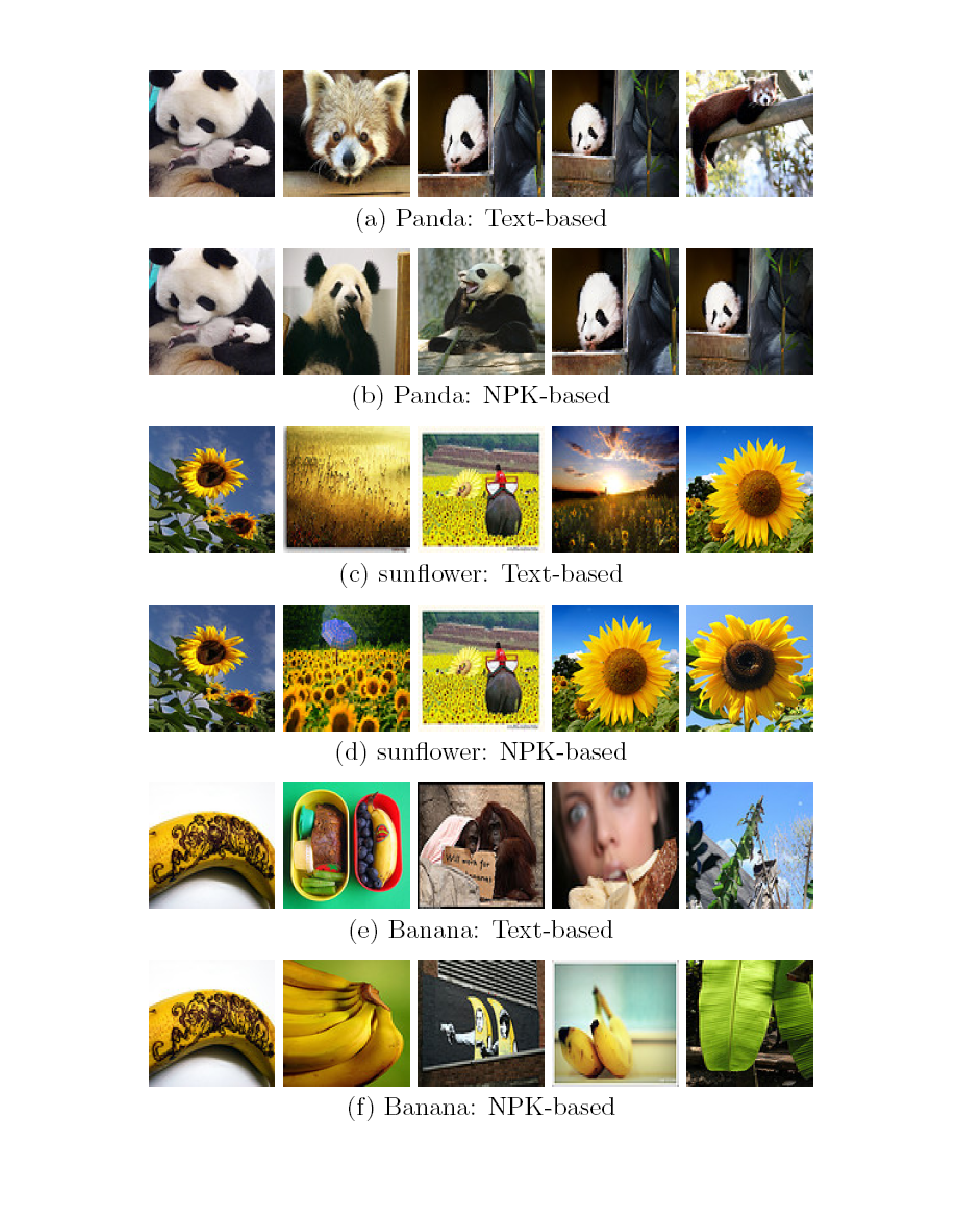
\includegraphics[width=5in]{figures/civr-results.eps}%\vspace{-0.4in}
\caption{Qualitative re-ranking performance by the proposed NPK learning method.} \label{fig:civr-illustration}
%\vspace{-0.2in}
\end{figure}


%========================================================
\subsection{Experiment II: Computational Cost}
%========================================================

The retrieval time is crucial for IR systems. In our non-parametric learning
framework, we propose a fast solution avoiding general semi-definite
programming solvers. In this section, we evaluate the time cost of the
following solvers:
\begin{itemize}
    \item {\bf SDP}: We solve (\ref{eqn:tk-dual}) using SDP solvers. However,
     the time complexity of SDP is in general $O(n^6)$, which prohibits
     the learning from real applications. Here we adopt the approximation
     method in Section \ref{sec:rerank-implementation} (see also
     \cite{nips/SongSBG07}).
    \item {\bf NPK}: The proposed method described in Algorithm \ref{alg:iterative-npk} with the same approximation scheme.
\end{itemize}

\begin{figure}[!ht]\label{fig:civr-time}
\begin{center}
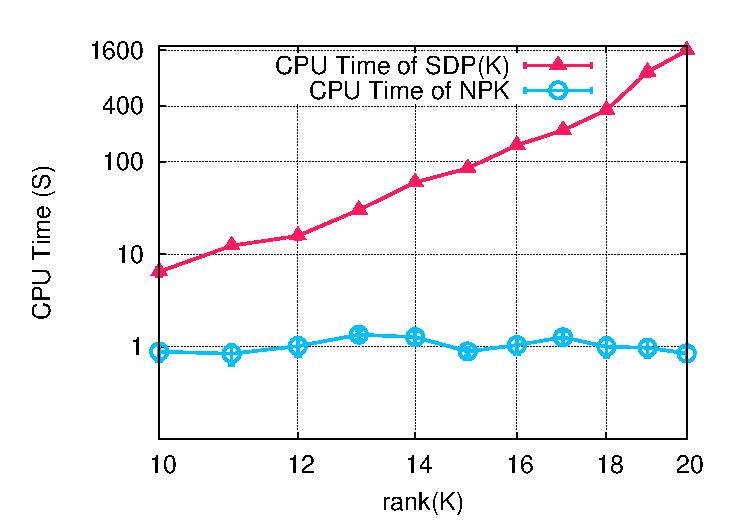
\includegraphics[width=5in]{figures/cvir_time.eps}
%\vspace{-0.2in}
\caption{Log-scaled computation time of SDP and NPK on the query {\em Big Ben} which contains 200 images with the
low-rank approximation scheme.}
\end{center}%\vspace{-0.3in}
\end{figure}

We plot the computational time of these two methods by Figure
\ref{fig:civr-time}. We draw the following two observations: 1) The NPK
method cost only around 1 second for a data set around 200 images, which
is practical for online applications. More importantly, the cost does not
crease with the rank significantly. For frequent queries, we could
pre-compute the ranking result and cache it to speed up the retrieval time
for real IR systems; 2) The complexity of SDP is verified by the
exponential shaped curve. As the rank increases, it becomes infeasible
easily.


%========================================================================
\section{Related Work} \label{sec:rerank-related-work}
%========================================================================

Our work is related to several branches of research topics: content-based
annotation and retrieval, text-based social image retrieval, and
nonparametric kernel learning.

Content-based methods for auto-image annotation and retrieval have been
extensively studied in multimedia area. The earlier studies on CBIR have
focused on investigating effective low-level features for image
representation~\cite{pami/SmeuldersWSGJ00}. While various
features have been proposed, effective CBIR methods remain a
challenging research problem till now, which is primarily due to the
well-known semantic gap between the low-level features and high-level
semantic concepts. To overcome the semantic gap challenge, much
research efforts have been paid on improving the interactive image
retrieval performance using relevance feedback techniques~\cite{tcsvt/RuiHOM98}. Our work is in general related to CBIR as we also exploit the visual contents of images, but is also different in that we
focus on improving text-based image retrieval performance without
explicit query image example while regular CBIR often focuses on solving
example-based image retrieval tasks without text.

In addition to CBIR, multimedia researchers have actively explored
content-based methods for auto-image annotation. By annotating an image
with some machine learning model automatically, we are able to enable a
large amount of unlabeled images indexed and searchable by existing text
based image search engines. a variety of techniques have been proposed
for auto-image annotation in recent
years~\cite{mm/DattaGLW06,sigir/WangZZ08,mir/LiuJYXSL08,mm/WuHJZY09}.
In general, auto-image annotation can be viewed as an intermediate task
for a generic web image retrieval task. Our work is however different from
the annotation-based retrieval approach, in that our focus is not on
improving the intermediate annotation performance, but for optimizing the
retrieval performance directly.

The text-based image retrieval problem is about to select images related to
a text query, which can be more clearly stated as: we rank the related
images $\{x^+\}$ on top of unrelated ones $\{x^-\}$ for a query $q$
according to their relevance score. Thus our work closely related to
learning to
rank~\cite{kdd/Joachims02,icml/BurgesSRLDHH05,nips/BurgesRL06,icml/CaoQLTL07,pami/GrangierB08}
and social image
retrieval~\cite{WIR03,MM04Cai,pami/JingB08,pami/GrangierB08,mm/HeLZTZ04,mm/DattaGLW06},
the goal of which is to learn a model that outputs an order over a set of
documents. For our proposed algorithm, we try to refining the results of
some ranking model instead of the ranking framework, though it could be
plugged into some kernel-based discriminative ranking model, like
\cite{pami/GrangierB08}. A lot of methods have been proposed for
improving regular text-based web image retrieval performance, including
re-ranking by relevance model~\cite{WIR03}, clustering based
re-ranking~\cite{MM04Cai}, and the VisualRank approach by modifying
PageRank~\cite{pami/JingB08}. Our work is mainly motivated by the
VisualRank approach for overcoming its limitation through a kernel based
learning approach, where a similarity matrix plays a central role for
propagating the ranking scores among images. Moreover, the learned
kernel can be plugged into other framework, for example,
\cite{pami/GrangierB08}.

Our algorithm closely relates to the subject {\em kernel
learning}\cite{jmlr/LanckrietCBGJ03}, which is enjoying great popularity
in machine learning community. Different from traditional parametric
kernel combinations~\cite{jmlr/LanckrietCBGJ03}, researchers have
proposed {\em nonparametric kernel learning} (NPK) algorithms, of
which the output is just the kernel matrix
\cite{icml/KulisSD06,icml/HoiJL07, icml/ZhuangTH09}. It is known that
each positive semi-definite kernel matrix $K$ (p.s.d.) corresponds to the
evaluation of some underlying Mercer kernel function $k: \X \times \X
\rightarrow \R$. Therefore, people never need to find the explicit
expression of $k$ in the transductive setting.

The most important merit of NPK is that it provides more flexibility to fit
the available data since it does not require any parametric function. It
often produces state-of-the-art empirical results for both classification and
clustering. To the best of our knowledge, there is no existing studies in
machine learning that have addressed web image retrieval by optimizing
kernel in the ranking task. Our work focuses on adapting the recent
advances of nonparametric kernel learning techniques with applications to
the social image ranking task. However, due to the p.s.d. constraint over
$K$, the learning often results in a semi-definite program~\cite{Boyd},
which has the time complexity of $O(N^6)$. Such heavy computation
makes NPK prohibitive for large scale application. Very recently, Zhuang
et. al. proposed an iterative algorithm which speeds up the kernel learning
significantly. Based on their work,  we derive an similar fast algorithm to
solve our optimization problem. Together with some tricks, it works for a
real data set consisting of more than 60,000 images.

%===============================================================
\section{Summary} \label{sec:rerank-conclusion}
%===============================================================

In this chapter, we present a novel nonparametric kernel ranking approach to an emerging application of social image retrieval. Unlike the previous studies that may considerably suffer from the semantic gap by some rigid visual similarity function for web image re-ranking, our new solution aims to overcome the semantic gap issue by learning an effective kernel from mining both textual tags and visual images in a unified optimization framework. Encouraging experimental results on a large social image testbed validates the efficacy of the proposed method. Future work will explore other more effective visual features, such as SIFT~\cite{jcv/LoweG04}, which poses a great challenge for being applied in a large-scale social image collection.






